\chapter{Decision Support in Connect Hydro}
\label{ChapterFour}
In the Last 2 chapters, We discussed the Decision support systems and all their features and the best techniques to develop them. We also introduced the Connect Hydro Project and discussed all its different ascpects. In this chapter we will discuss what kind of decision support system could be implemented within the connect hydro project and how it can bring an added value. Our solution is based on the work already implemented in the connect hydro prototype. In our project, we implemented a simple DSS system integrated in a web portal.

The Application flow starts as follows: Data from sensors at the power plants is gathered as well as sensor data from external sources and stored in the central system , mainly in the database. From this database, the knowledge processing system can learn, based on the events defined in the event matrix, e.g. how several sensor data combinations and occurrences will lead to which events. Based on the knowledge in the system, it is possible to predict harmful occurrences (e.g. a flooding of a power plant can damage the active turbines) or apply a set of predefined rules to the processed data, to make decisions. An example of decision to propose is to pdeactivate the turbines when a flooding is predicted and give signals either to the early warning system (e.g. message to the owner/operator of the small hydro power plant that it is recommended to deactivate the turbines) or an installed regulation system (e.g. which automatically can deactivate the turbines).\cite{SEIT2017}

\section{Connect Hydro DSS Type}
In \textit{ChapterTwo} we discussed how a DSS system should be designed, starting with the problem definition in terms of input, output, user knowledge/expertise and decisions. In connect Hydro, the DSS's problem is to optimize the energy production of one power plant using the data received from downstream and upstream power plants, historical data as well as external resources. To solve this problem we would like to explore the possibilty of combining two types of Decision support systems, the data-driven and the knowledge-driven systems as each seperately prove exteremely beneficial in solving our problem.

\textbf{The data-driven approach} would prove to be very efficient in managing the huge amounts of sensor data as well as the data from the external sources. The external sources can include weather forecasts, historical data of events etc..The historical data can be analyzed using an On-line Analytical Processing (OLAP) tool which will definetly contribute with producting in a fast manner decisions that were evaluated from every aspect to the power plant owners.

\textbf{The knowledge-driven approach} is also an effective approach for our problem. Part of the information that should be provided by the power plant owners would be a set of their rules. These rules can either be power plant specific or general rules applied to all power plants along the "Alm" river, depending on the agreement between the power plants. An example rule would be "If Water Level > 'Defined Threshold', Turn off the Turbines."

Both approaches alone are very relevant to our problem and would prove very efficient, but we think combining them would provide better results. In the next section we will discuss the event matrix that was proposed for our system.

\section{Connect Hydro Event Matrix}
In our portal, we chose only a few events to model as well as sensor data from November 2016 for 3 power plants. The sensor data were extracted from the database of connect hydro project. The sensors that were used for our prototype included:\\
\begin{center}
\begin{tabular}{ |c| } 
 \hline
 Sensor\\ [0.5ex] 
 \hline\hline
Water opening Size\\ 
Power output turbine\\ 
Water level at turbine\\ 
Water level after rack \\ 
Water level before rack\\ 
Canal Closed at rack\\
Canal Opened at rack\\
Cloudiness \\
Rack Cleaning\\
 \hline
\end{tabular}
\end{center}
Using the data from these sensors for the powerplants, we came up with an event matrix. The event matrix is the events that can happen if a combination of values from different sensors occur. In our prototype we considered 4 Events, the water temperature, water level, Turbidity and the lack energy output. The 4 events are described below:\\
\begin{itemize}
	\item \textbf{Flooding:} if the water level rises above a predefined threshold, the water channel should be closed, so that the turbines are not damaged due to the high amount of water. Reaction: Turn down/off Turbine \& Activate Rack Cleaner.
	\item \textbf{Low water level:} if the water level in the water channel falls below a predefined threshold, the turbines cannot work properly. The water-supply should be regulated so that the turbines can work with a lower capacity and there won't be any downtime of the turbine. Reaction: Regulate Turbine.
	\item \textbf{Waste dump:} if the turbidity of the water is very high, it could be that there is so much dirt, which can damage the turbines. The turbines should be turned off, so the water channel can be cleared from dirt. Reaction: Turn off Turbine \& Activate Rack Cleaner.
	\item \textbf{Ice:} if the water temperature falls below a predefined threshold, it is possible that ice will appear at the rack, which could lead into a frozen water channel. Reaction: Turn on Rack Heating.
	\item \textbf{No Energy output:} if the water level at the previous power plant downstream is low and they dont have any energy output, then water level will be also low at my power plant. Reaction: Turn off Turbine \& Close Down Water Canal.
	\end{itemize}
A visualization of the event matrix was included in the web portal as shown in the following figures.
\begin{figure}[H]
\centering
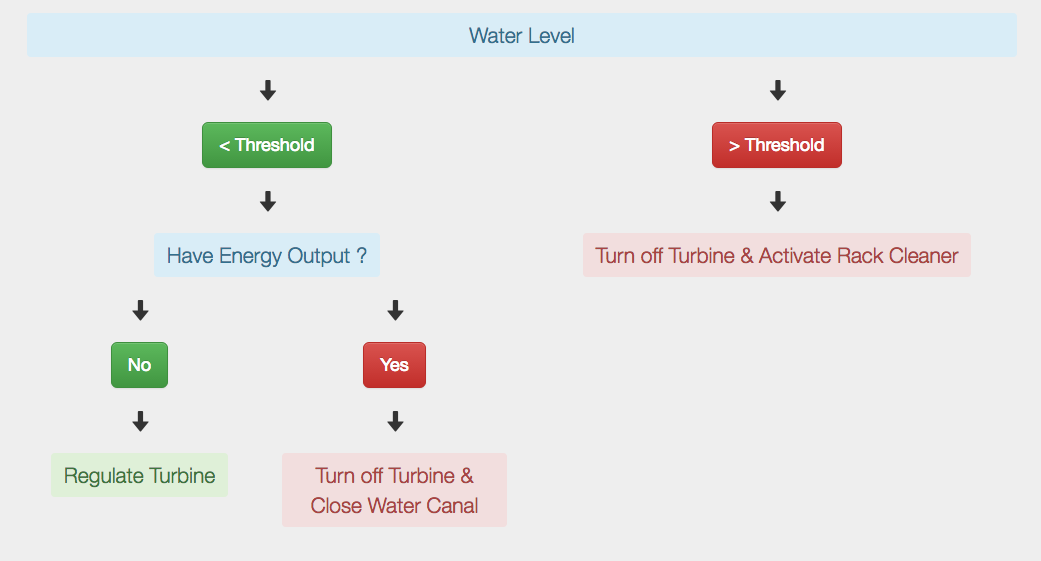
\includegraphics[scale=0.4]{Images/WaterLevel.png}
\caption[Low water Level, No Energy output and Flooding Events]{Low water Level, No Energy output and Flooding Events}
\end{figure}
Figure 4.1 explains how the events of the "Low Water Level", "No Energy Output" and "Flooding" were modelled.
\begin{figure}[H]
\centering
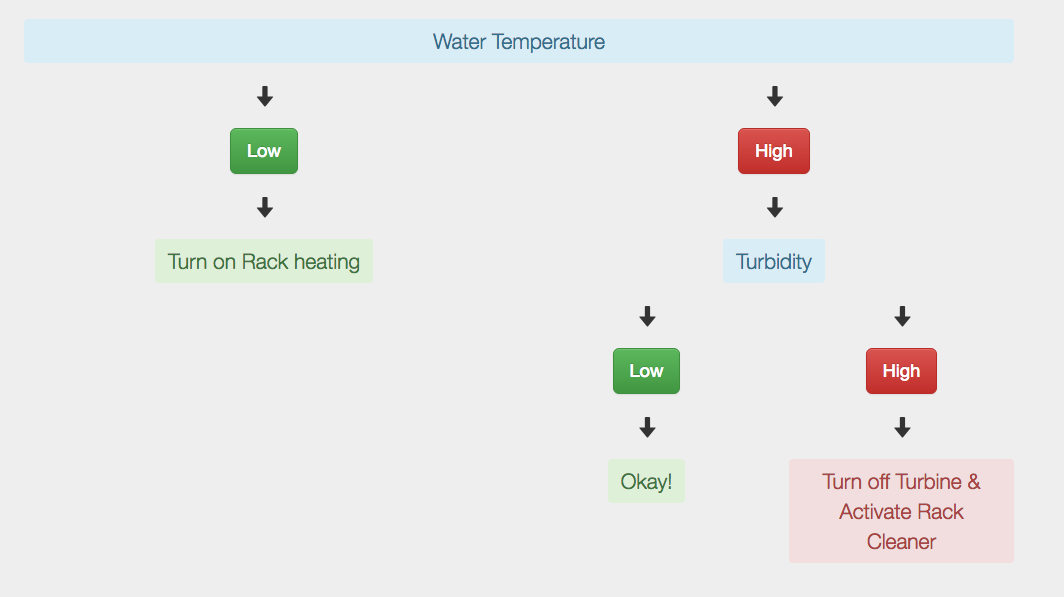
\includegraphics[scale=0.4]{Images/WaterTemperatureAndTurbidity.png}
\caption[Waste Dump and Ice Events]{Waste Dump and Ice Events}
\end{figure}
Figure 4.2 explains how the events of the "Waste Dumo" and "Ice" were modelled.
In the next section we will discuss our approach in designing and Implementing the Connect Hydro DSS as well as the limitations we faced and what could be future enhancements that would make the system even more useful.
\section{Connect Hydro DSS Design \& Implementation}
In Chapter two, We mentioned that there should be four components properly defined before we can proceed into the designing and implementing processes.
\begin{itemize}
	\item Input: Input for connect hydro DSS would be the sensor data coming from the power plant, historical data saved in the database and data from external resources (e.g. Weather Forecast).
	\item User Knowledge/Expertise: No user expertise will be needed in forming the decisions, but the users will need to implement the decisions.
	\item Output: The output will be specific for every powerplant.
	\item Decisions: The system will suggest actions to power plant owners after analyzing the data and determine the needed action to correspond to the input.
\end{itemize}
After Defining the problem, the next step would be to start Analyzing the DSS from a business prespective and deciding what type of decisions the DSS will provide. In our prototype, The DSS will support operational decisions, decisions that impact the day-to-day activities as well as contribute to the overall goal of increasing the energy production for the small power plants. The decisions to be produced by our DSS will be repetitive as well as structured, the sitiuation doesnt drastically change from 1 day to the other and the possible outcomes are limited.

The next step after analyzing the business prespective would be to define the problem solving process.
\begin{itemize}
	\item 1. Defining the Problem: The problem is to provide decisions for power plant owners to maximize their energy production and minimize downtime for the power plant.
	\item 2. Identifying Decision Maker: The decision maker is the owner of the power plant.
	\item 3. Gathering Information: Data will be collected from sensor data at the power plant as well as the previous power plants, historical data saved in the database and finally external resources.
	\item 4. Evaluating Alternatives and Deciding: The system will evaluate all the data and try to see if the data matches any of the predefined events in the event matrix or if any of the rules defined by the power plant owner are applicable and decide the best action that the owner should do.
	\item 5. Implementation and Follow-up: There should be a system keeping track of the actions taken and if the decided actions were implemented by the owner and be used as part of the historical data to be used in the future decision making.
\end{itemize}
In development of our DSS, we used SDLC - System Development Life Cycle Approach. Although SDLC is the most rigid system development approach, it fit the needs of this project as it was just a prototype. In the future, we beleive the Rapid Prototyping Approach will be better and the involvement of the end users will definetly bring an added value to the project and motivate them to use the system.

The Connect Hydro DSS user Interface was a simple Interface which starts the decision making process on demand and the result was presented to the user as simple to-do list of all the actions that should be taken. Visualization of sensor data was also included as a modeule to further convince the owners that the decisions produced by the DSS are valid and aim to make them more profitable till they could trust the software.
\section{Visualization for Connect Hydro}
In Connect Hydro, Data Visualization was included as a tool to further convince the power plant owners that the decisionns produced by the DSS were correct with the final goal of maximizing their energy production. The visualizations produced included 2 different Line charts. The first chart showed how the Energy output differed depending on the Water Level. The second chart showed the energy production of one power plant over time. Examples of the 2 charts are shown below in Figures 4.3 and 4.4.
\begin{figure}[H]
\centering
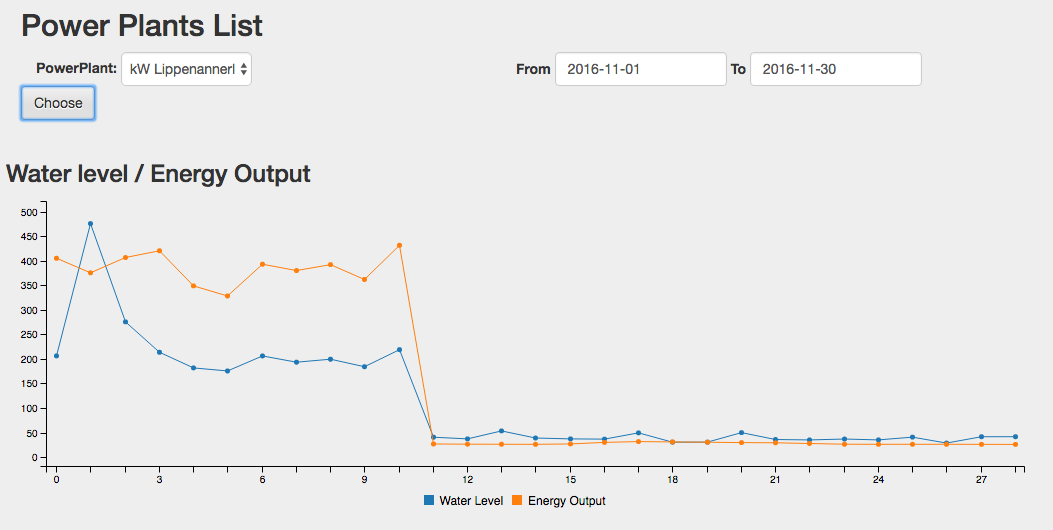
\includegraphics[scale=0.4]{Images/Chart1.png}
\caption[Water Level/Energy Output per day]{Water Level/Energy Output per day}
\end{figure}
\begin{figure}[H]
\centering
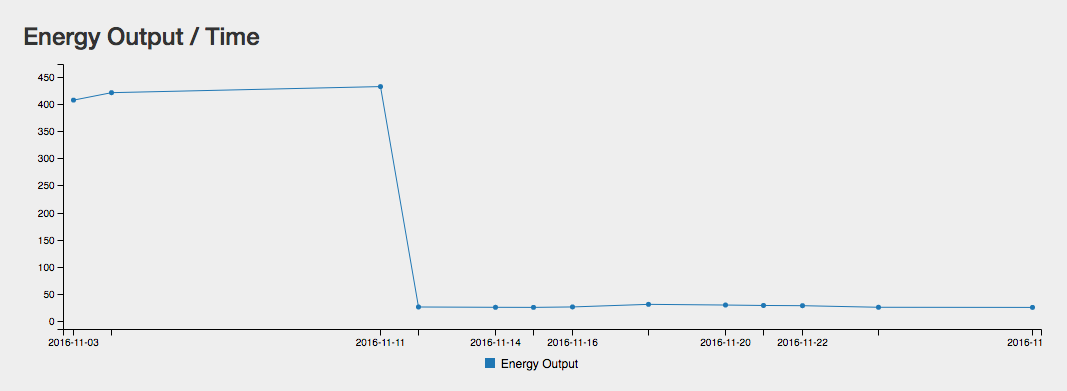
\includegraphics[scale=0.4]{Images/Chart2.png}
\caption[Energy Output per day]{Energy Output per day}
\end{figure}